\let\negmedspace\undefined
\let\negthickspace\undefined
\documentclass[journal]{IEEEtran}
\usepackage[a5paper, margin=10mm, onecolumn]{geometry}
%\usepackage{lmodern} % Ensure lmodern is loaded for pdflatex
\usepackage{tfrupee} % Include tfrupee package

\setlength{\headheight}{1cm} % Set the height of the header box
\setlength{\headsep}{0mm}     % Set the distance between the header box and the top of the text

\usepackage{gvv-book}
\usepackage{gvv}
\usepackage{cite}
\usepackage{amsmath,amssymb,amsfonts,amsthm}
\usepackage{algorithmic}
\usepackage{graphicx}
\usepackage{textcomp}
\usepackage{xcolor}
\usepackage{txfonts}
\usepackage{listings}
\usepackage{enumitem}
\usepackage{mathtools}
\usepackage{gensymb}
\usepackage{comment}
\usepackage[breaklinks=true]{hyperref}
\usepackage{tkz-euclide} 
% \usepackage{gvv}                                        
\def\inputGnumericTable{}                                 
\usepackage[latin1]{inputenc}                                
\usepackage{color}                                            
\usepackage{array}                                            
\usepackage{longtable}                                       
\usepackage{calc}                                             
\usepackage{multirow}                                         
\usepackage{hhline}                                           
\usepackage{ifthen}                                           
\usepackage{lscape}
\begin{document}

\bibliographystyle{IEEEtran}
\vspace{3cm}

\title{9.3.12-D}
\author{EE24BTECH11029 - J SHRETHAN REDDY}
\maketitle
% \newpage
% \bigskip
{\let\newpage\relax\maketitle}

\renewcommand{\thefigure}{\theenumi}
\renewcommand{\thetable}{\theenumi}
\setlength{\intextsep}{10pt} % Space between text and floats


\numberwithin{equation}{enumi}
\numberwithin{figure}{enumi}
\renewcommand{\thetable}{\theenumi}

\textbf{Question}:\\
Solve the following differential equation:

\begin{align}
 \frac{d^2y}{dx^2} + x \frac{dy}{dx} + xy &= 0
\end{align}
\solution

By first principle of derivatives,
\begin{align}
    y^{\prime}(t) &= \lim_{h\to 0}\frac{y(t+h) - y(t)}{h} \\
    y(t+h) &= y(t) + hy^{\prime}(t)
\end{align}

\begin{align}
 \frac{d^2y}{dx^2} + x \frac{dy}{dx} + xy &= 0
\end{align}

Rewriting the given equation, we get:
\begin{align}
\frac{d^2y}{dx^2} &= -x \frac{dy}{dx} - xy
\end{align}

To solve this equation numerically, we apply Euler's method. We start by introducing the following substitutions:

Let:
\begin{align}
y_1 = y, \quad y_2 = \frac{dy}{dx}
\end{align}

Thus, the system becomes:
\begin{align}
y_1^\prime &= y_2
\end{align}
\begin{align}
y_2^\prime &= -xy_2 - xy_1
\end{align}

The system of equations in matrix form:
\begin{align}
\vec{y^\prime} &= \begin{bmatrix} 
y_2 \\ 
-xy_2 - xy_1 
\end{bmatrix}
\end{align}

Using Euler's method, the update formulas become:
\begin{align}
y_1(x+h) &= y_1(x) + h \cdot y_2(x)
\end{align}
\begin{align}
y_2(x+h) &= y_2(x) + h \cdot \left( -xy_2 -x y_1 \right)
\end{align}

This can be expressed in matrix form as:
\begin{align}
    \vec{y}_{n+1} &= \vec{y}_n + h \begin{bmatrix}
    0 & 1 \\ 
    -x & -x 
    \end{bmatrix} \cdot \vec{y}_n
\end{align}

We will assume two initial conditions:
\begin{align}
x_0 = 0,\quad y_0 = 0
\end{align}
substitute above initial condition in the eq(0.10) and eq(0.11) ..so on we will get all other y values 
Now, applying Euler's method and iterating, we obtain the numerical solution. The following plot represents the solution based on these initial conditions.

 \begin{figure}[h!]
    \centering
    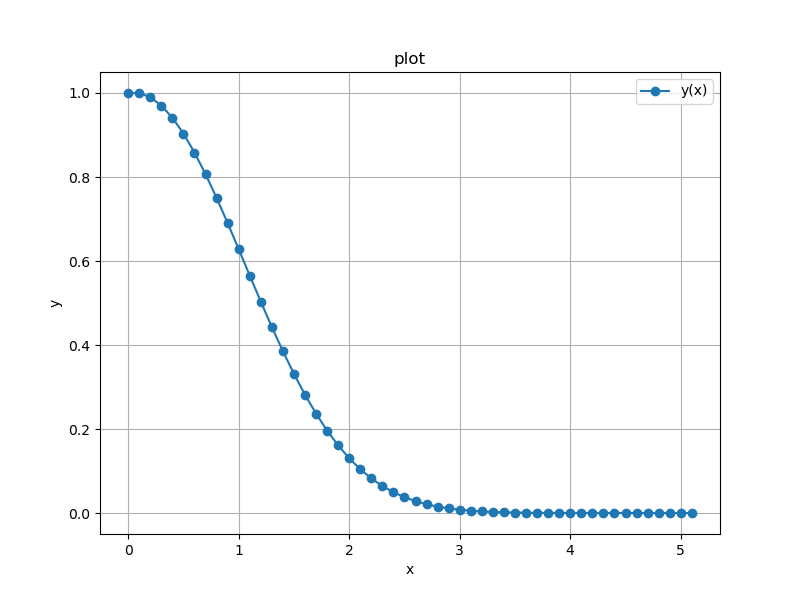
\includegraphics[width=1\columnwidth]{figure/fig.png} 
    \caption{Numerical Solution}
    \label{stemplot}
\end{figure}

\end{document}

